\chapter{Phase de développement~: conception et implémentation d'un module
statistique}
	\paragraph{}
	Dans la partie précédente nous avons proposé une solution fonctionnelle aux
	besoins exprimés par les utilisateurs. Ici, nous allons concevoir la solution
	technique qui en découle, puis l'implémenter
	c'est-à-dire en écrire le code.
	La partie A présentera l'architecture actuelle de TrackCIS. La partie B
	présentera la conception de la solution technique. La partie C présentera
	la méthodologie d'implémentation de cette solution. Enfin, dans la partie D, nous ferons le
	bilan de ce qui a effectivement pus être développé au cours de ce projet et
	nous discuterons des limites et des biais de la méthodologie ainsi que des
	suites possibles pour Xperis.
	
	\section{TrackCIS, une application web en deux parties}
		
		\subsection{Qu'est-ce qu'une application web ?}
			\paragraph{}% Modèle client serveur classique
			TrackCIS est une application accessible depuis un navigateur internet, il
			s'agit d'une application web. Classiquement, le fonctionnement de ce type
			d'application est basé sur le modèle dit <<client-serveur>>. Un client
			correspond au navigateur internet de l'utilisateur (Chrome, Firefox\ldots),
			il permet de communiquer avec le serveur. Ce dernier est une machine sur
			laquelle est déployée l'application web. Le client envoie une requête au
			serveur qui va la traiter et générer en retour une page web au format HTML
			(Hypertext markup language) qui est renvoyée au client puis affichée
			(figure \ref{client_serveur}). La requête utilise le protocole HTTP
			(Hypertext transfert protocole) qui est le protocole standard des échanges
			sur le net. La page HTML contient toutes les informations permettant au
			navigateur d'afficher la page. Cette page peut faire appel à d'autres
			ressources comme des fichiers CSS (Cascading style sheets) ou des script
			Javascript. CSS est un langage descriptif permettant de mettre en forme le
			contenu de la page HTML.
			Javascript est un langage qui est interprété par le navigateur et qui
			permet de gérer les éléments dynamiques de la page web (animations, gestion
			des événements lorsque l'utilisateur clic sur un bouton\ldots).
			\begin{figure}[H]
				\centering
				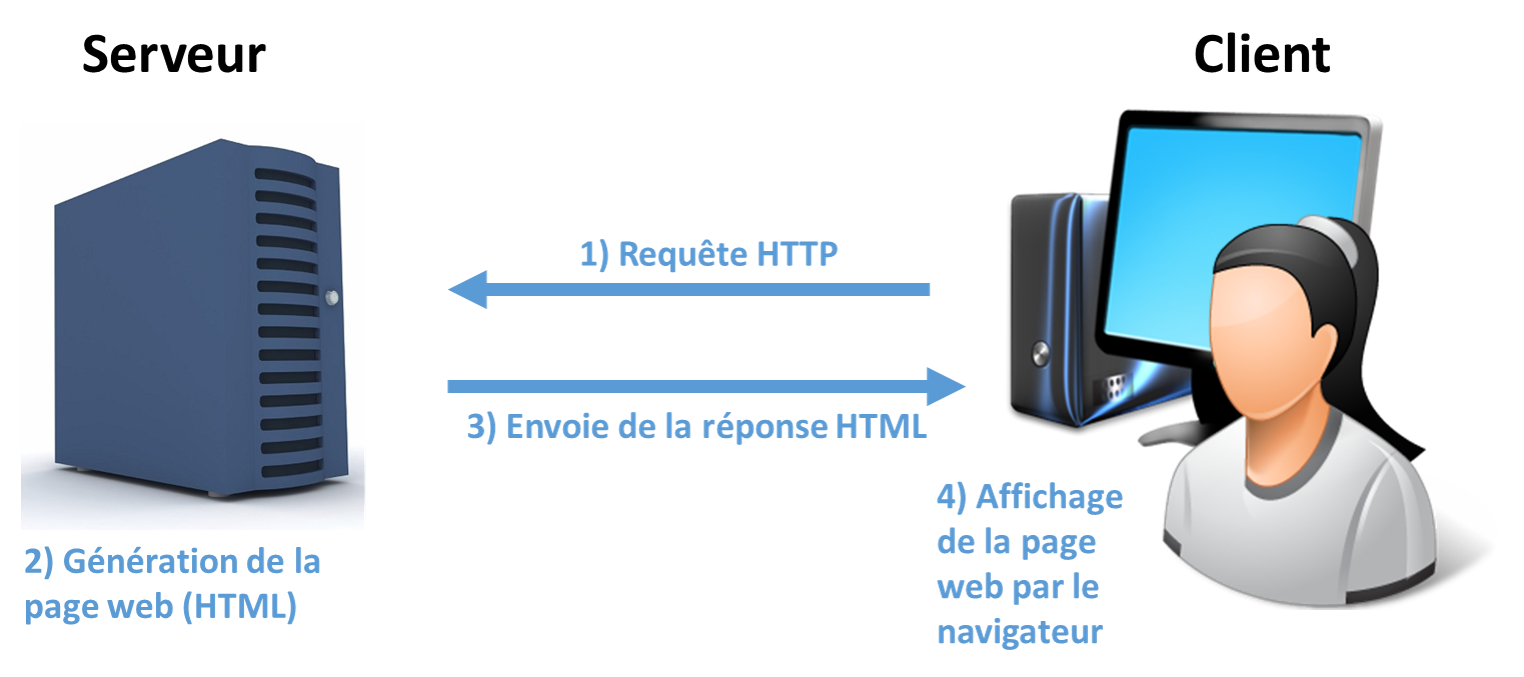
\includegraphics[width=10cm]{../img/part3/client_serveur.png}
				\caption{\label{client_serveur} Le serveur génère dynamiquement la page
				HTML qui sera affichée sur le poste client.}
			\end{figure}
			
			\paragraph{}% Modèle AJAX
			Une variante du modèle client-serveur permet d'en augmenter la rapidité, il
			s'agit du modèle AJAX (Asynchronous javascript and XML).
			Le modèle précédent implique que toute la page doit être renvoyée par le
			serveur à chaque requête, ce qui n'est pas forcément nécessaire. Cela pose
			deux problèmes :
			d'une part beaucoup de données transitent entre le client et le serveur,
			d'autre part le rechargement complet de la page prend du temps ce qui nuit à
			l'expérience de l'utilisateur.
			Le modèle AJAX, sur lequel repose en grande partie TrackCIS, consiste à ne
			recharger que les parties de la page qui sont concernées par la modification
			sans toucher au reste.
			Prenons l'exemple d'une page affichant la liste des messages entre
			une date de début et une date de fin. Si l'utilisateur modifie la période,
			seule la partie correspondant à la liste des messages sera rechargée. Le
			reste de la page (menu, pieds de page, entête\ldots) ne sera pas renvoyé par
			le serveur. Les appels AJAX sont réalisés au niveau des scripts Javascript,
			donc côté client.
			
		\subsection{TrackCIS est composé d'un frontal et d'une API}
			\paragraph{}% Archi générale de l'application
			TrackCIS repose sur les deux précédent. Les deux
			premiers éléments de l'architecture sont le client (le navigateur internet
			de l'utilisateur) et le serveur hébergeant l'application web stricto-sensu,
			que nous appelerons dans la suit le <<Frontal>> (figure
			\ref{archi_trackcis}).
			Le Frontal reçoit et traite les requêtes envoyées par le client. Il
			ne communique pas directement avec Cloverleaf, c'est une autre partie de
			l'architecture qui s'en charge : l'API.
			API signifie Interface de programmation applicative. D'une façon générale,
			une API sert d'intermédiaire entre deux applications. Dans notre cas, l'API est
			l'intermédiaire entre le Frontal, qui a pour but d'afficher la page web, et
			Cloverleaf. Prenons un exemple : le client envoie une requête au Frontal
			pour afficher la liste de tous les messages passé sur un flux donné durant
			une période donnée. Le Frontal reçoit la requête et envoie à son tour une
			nouvelle requête à l'API.
			L'API récupère les informations demandées auprès de Cloverleaf et
			les transmet au Frontal. Enfin, celui-ci génère la page HTML avec la liste
			des messages qui a été demandée et l'envoie au client.\newline
			API et Frontal sont deux entités séparées, toutes deux développées par
			Xperis. Ils ne sont généralement pas déployés sur le même serveur. L'API est
			nécessairement installée sur le même serveur que Cloverleaf, le Frontal est
			quant à lui habituellement installé sur un serveur à part situé au
			sein de l'établissement hospitalier d'un serveur.
			\begin{figure}[H]% Architecture globale de l'application
				\centering
				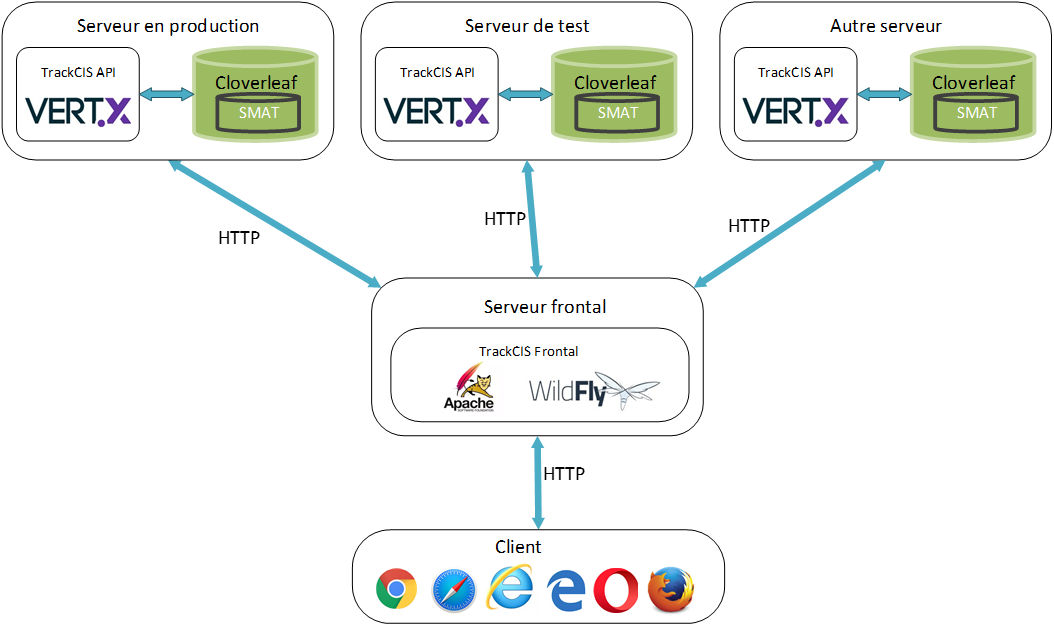
\includegraphics[width=10cm]{../img/part3/archi_trackcis.png}
				\caption{\label{archi_trackcis} TrackCIS est composés de deux éléments
				distincts pouvant se trouver sur deux serveurs différents.}
			\end{figure}
			Frontal et API sont tous deux développés avec le langage Java.
			
		\subsection{Le frontal est développé en java J2EE}
			\paragraph{}% les grandes lignes de l'archi du front
			Java entreprise édition, que nous désignerons par J2EE, est une
			plateforme basée sur le langage Java et destinée au développement web. Il
			s'agit d'un ensemble de bibliothèques Java mettant à disposition des
			développeurs les éléments nécessaires au développement d'une application
			web.
			
			\paragraph{}
			Java a la particularité d'être un langage orienté objet. Le code est organisé
			en classes. Une classe peut posséder un certain nombre d'attributs
			(données stockées sous la forme de variables) et de méthodes (opérations
			que la classe est capable d'effectuer). La classe peut contenir des données
			et des traitements. La figure \ref{archi_actuelle_front} résume
			l'architecture actuelle du Frontal de TrackCIS. Chaque bloc sur le schéma représente un
			groupe de classes ayant des rôles similaires. Globalement, le Frontal
			respecte l'architecture dite MVC (Modèle, contrôle, vue) qui permet de
			diviser le code selon trois grands rôles : les traitements (Modèle) la
			génération de la page HTML (la Vue) et des classes faisant office
			d'intermédiaire entre Modèle et Vue (les Contrôleur). (1) La requête HTTP
			envoyée par le client et reçue au niveau des classes dites <<contrôleur>>.
			Ces classes n'effectuent presque pas de traitement et ne se contentent que de
			faire appel aux classes de services.
			Celles-ci effectuent les opérations les plus complexes (2). Les classes de
			répertoire (ou repositories) permettent de communiquer avec la base de
			données (3).
			Cette dernière permet de stocker les préférences des utilisateurs ainsi que
			d'autres données de paramétrage (adresse du serveur de
			Cloverleaf, port utilisé\ldots). Les classes de répertoire permettent
			d'envoyer des requêtes SQL à cette base de données pour en lire les
			informations ou les mettre à jour. Les classes de données (4) contiennent
			essentiellement des attributs et peu de méthodes. Comme leur nom
			l'indique elles permettent de stocker des données comme par exemple celles
			récupérées par les répertoires depuis la base de données, ou bien les
			données renvoyées par l'API (6). Certaines classes de services (5)
			permettent d'envoyer des requêtes HTTP à l'API et d'en recevoir la réponse.
			Cette réponse contient les données demandées par l'utilisateur qui sont
			ensuite stockées dans une classe de donnée. Enfin, la vue (7), c'est-à-dire
			la page HTML, est générée grâce à la technologie JSP (Java server pages). Il
			s'agit d'un langage proche du langage HTML permettant de générer
			dynamiquement une page HTML.
			Les pages JSP permettent de mettre en forme et d'afficher les données reçues
			de l'API. C'est le contrôleur qui met les données à disposition de la JSP.
			\begin{figure}[H]
				\centering
				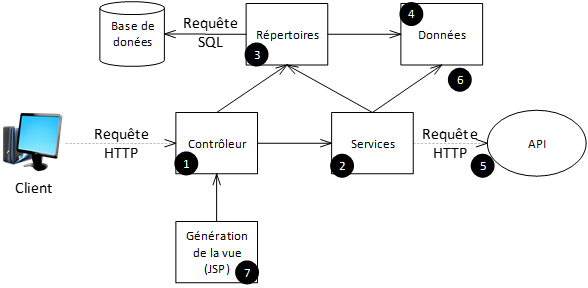
\includegraphics[width=10cm]{../img/part3/archi_actuelle_front.png}
				\caption{\label{archi_actuelle_front} Architecture simplifiée du Frontal
				de TrackCIS. Les flèches continues représentent les dépendances entre les
				éléments.}
			\end{figure}
			
		\subsection{L'API permet de communiquer avec Cloverleaf}
			\paragraph{}% Les grandes lignes de l'archi de l'API
			L'API est développée grâce à la plateforme standard de Java ou Java SE
			(Standard édition) qui n'est pas destinée au développement web. En effet
			l'API n'est pas une application web, il s'agit d'un petit programme Java qui
			s'execute sur le même serveur que Cloverleaf et qui permet d'intéragir avec
			l'EAI. L'API est capable de reçevoir et d'interpréter des requêtes
			HTTP, ce qui est rendu possible grâce à la technologie Vertx. Il s'agit
			d'un ensemble de bibliothèques permettant mettant à disposition des
			développeurs des outils pour gérer la réception de requêtes HTTP.
			
			\paragraph{}
			On retrouve dans l'API des éléments similaire à ceux du Frontal. Tout d'abord
			une classe jouant le rôle de contrôleur permet de récupérer la requête HTTP
			envoyée par le Frontal et d'envoyer une réponse (figure
			\ref{archi_actuelle_api}, (1)). La réponse contient toutes les données
			demandées par la requête, pour la construire le contrôleur fait appel à des
			classes de services (2). Celles-ci vont se connecter à Cloverleaf et
			récupérer les informations demandées dans certaines bases de données de l'EAI. Les
			classes de services vont ensuite faire appel aux classes de données pour
			stockées les informations (3). Ce sont ces dernières qui vont permettre au
			contrôleur de construire la réponse.
			\begin{figure}[H]
				\centering
				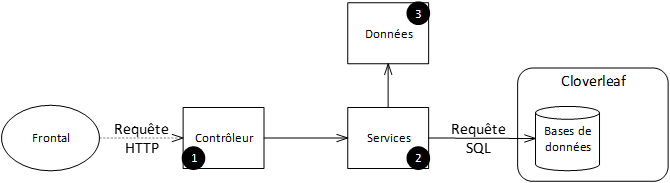
\includegraphics[width=9cm]{../img/part3/archi_actuelle_api.png}
				\caption{\label{archi_actuelle_api} Architecture simplifiée de l'API de
				TrackCIS.}
			\end{figure}
	
	\section{L'analyse technique permet d'implémenter le nouveau module sur la base
	de l'existant}
		\paragraph{}
		A présent que nous savons comment est construit TrackCIS, nous pouvons
		commencer la conception du module statistique. Cette phase précède le
		développement à proprement parler. Son but est de définir tous les
		éléments techniques qui composerons le module, à savoir :
		\begin{itemize}
		  \item L'architecture, autrement dit la manière dont le code est structuré
		  \item Les outils utilisés, les bibliothèques, Framework\ldots
		  \item Le modèle de données, c'est-à-dire la structure de la base de données
		\end{itemize}
		La principale contrainte est de nous adapter à l'architecture existante. Nous
		souhaitons y <<greffer>> le module statistique sans pour autant changer ce qui
		a déjà été mis en place que ce soit au niveau de l'API, du Frontal ou de la
		base de données.
		
		\subsection{Un module qui est basé sur les données disponibles dans
		Cloverleaf}
			\paragraph{}
			Les statistiques qui nous intéressent sont des données sauvegardées
			automatiquement et à intervalles réguliers par l'EAI
			dans des bases de données. Dans Cloverleaf, les process sont regroupés en
			sites et les statistiques sont sauvegardé par site. Il existe une base de
			données pour chacun d'eux. Il s'agit de base de données SQLite. SQLite est un
			type de base de données qui se présente sous la forme d'un simple fichier.
			L'inconvénient est qu'il ne peut pas contenir un volume trop important de
			données. C'est pourquoi Cloverleaf crée un nouveau fichier SQLite dès que le
			précédent est plein.
			
			\paragraph{}
			Les données sont organisées en tables, comme dans une base de données
			classique. Les bases de données dont il est question ici sont intrinsèques
			à Cloverleaf et nous n'avons pas la main dessus. Elles constituent les
			sources de données auxquelles nous allons nous connecter. Il nous est
			impossible d'en modifier la structure et les seules requêtes que nous
			effectuerons sur ces tables sont des requêtes de lecture.
			
			\paragraph{}
			Dans chaque base SQLite il y a cinq tables, chacune représentant
			un niveau de détail :
			\begin{description}
			  \item[Host :] Cette table contient les données relatives au serveur
			  Cloverleaf. Sont sauvegardés ici à intervalles réguliers l'espace
			  disponible sur le disque ou l'état de la mémoire vive
			  \item[Site :] Cette table ne contient qu'une seule ligne (un seul
			  enregistrement) qui décrit le site correspondant à la base de données : nom
			  du site, nom de l'hôte sur lequel il est installé
			  \item[Process :] Cette table contient des données enregistrées à
			  intervalles régulier et qui renseigne sur le bon fonctionnement du process
			  (c'est-à-dire du bon fonctionnement de l'ensemble des Threads qui le
			  compose). On y trouve deux informations : l'état du process (arrêté, en
			  marche, en erreur\ldots) et la liste des threads qui le compose (sous la
			  forme d'une chaine de caractères)
			  \item[Thread :] La table Thread est celle qui nous intéresse le plus dans
			  ce projet puisqu'elle contient un grand nombre d'informations sur chaque
			  thread de l'ensemble du site. A la suite de l'analyse fonctionnelle nous
			  avons déterminé un certain nombre de statistiques qu'il serait intéressant
			  d'afficher à l'utilisateur de TrackCIS. Le tableau \ref{donnees_threads}
			  présente, pour chaque type de statistiques, les données dont nous avons
			  besoin et qui se trouvent dans la table Thread.
			  \item[Interthread :] Cette dernière table contient des informations
			  concernant chaque paire de thread. A chaque sauvegarde des statistiques par
			  Cloverleaf, autant d'enregistrement (autrement dit de lignes) sont créées
			  dans cette table que de paire de thread possible pour ce site. Cette table
			  ne nous sera pas utile pour les statistiques que nous souhaitons afficher.
			\end{description}
			La plupart des tables (c'est-à-dire toutes sauf la table Site) il existe une
			colonne qui contient la date et heure d'enregistrement.
			\begin{table}[H]
				\centering
				\caption{\label{donnees_threads} Lien entre les données que nous
				souhaitons afficher à l'utilisateur de TrackCIS et les données disponibles
				dans Cloverleaf.}
				\begin{tabular}{| p{5cm} | p{8cm} |}
					\hline
						\thead{Type de statistique}
						&\thead{Données dans la table Thread}
						\\
					\hline
						Historique du nombre de message
						&
						Données issues de la table Thread :
						\begin{itemize}
						  \item Nombre de messages entrant et sortant de chaque thread
						  \item Nombre de messages en attente
						  \item Nombre de messages en erreur
						\end{itemize}
						\\
					\hline
						Temps de transfert moyen d'un message dans un flux donné
						&
						Données issues de la table Thread :
						\begin{itemize}
						  \item Temps de transfert total
						  \item Nombre de messages en sortie du flux (pour pouvoir calculer une
						  moyenne par message ayant transité dans le flux)
						\end{itemize}
						\\
					\hline
						Taux de disponibilité d'un flux (temps de bon fonctionnement divisé par le
						temps total)
						&
						Données issues de la table Thread :
						\begin{itemize}
						  \item Date de dernier démarrage du thread
						  \item Date de dernier arrêt du thread
						  \item Etat du protocole à un instant donné
						  \item Date de dernière erreur de protocole
						\end{itemize}
						\\
					\hline
						Etat des ressources du serveur (mémoire vive, disque dur\ldots)
						&
						Données issues de la table Host :
						\begin{itemize}
						  \item Espace total du disque dur
						  \item Espace libre sur le disque dur
						  \item Quantité de mémoire vive total du serveur
						  \item Quantité de mémoire vive libre
						\end{itemize}
						\\
					\hline
						Historique de l'occupation du disque du serveur Cloverleaf
						&
						Données issues de la table Host :
						\begin{itemize}
						  \item Espace total du disque dur
						  \item Espace libre sur le disque dur
						\end{itemize}
						\\
					\hline
				\end{tabular}
			\end{table}
		
% >>>>>>>>>>>>>>>>>>>>>>>>>>>>>>>>>>>>>>>>>>>>>>>>>>>>>>>>>>>>>>>>>>>>>>>>>>>>>>>>>>>>>>>>>>
		
		\subsection{Nouvelle architecture de l'application}
			\paragraph{}% Une archi dessinée à partir des contraintes fonctionnelles
			La conception du module statistique de TrackCIS doit respecter les
			contraintes suivantes~:
			\begin{itemize}% Liste des contraintes
			  \item être basé sur l'architecture déjà en place. Il n'est pas question
			  dans ce projet de faire des modifications de l'existant. Ceci est
			  valable aussi bien pour le code lui-même que pour la structure de la base
			  de donnée.
			  \item être fermé à la modification et ouvert à l'extention. C'est-à-dire
			  qu'il doit être possible, pour une équipe de développement ultérieur,
			  d'ajouter des fonctionnalités au module sans avoir à modifier le code
			  existant (simplement en ajoutant des classes).
			  \item ne pas perturber le fonctionnement de Cloverleaf. Pour afficher des
			  données pertinentes pour l'utilisateur, certains traitements seront
			  nécessaires sur les données brutes. Ceux-ci peuvent cependant ralentir ou
			  perturber le fonctionnement de Cloverleaf. Il est nécessaire pour cela que
			  ces traitements ne soient pas fait sur le serveur de l'EAI, donc pas au
			  niveau de l'API.
			  \item ne pas surchager le serveur sur lequel est déployé le Frontal. Le
			  serveur servant à héberger le frontal n'est pas forcément une machine très
			  puissante, bien que cela varie en fonction des établissements.
			\end{itemize}
			
			\paragraph{Changements au niveau du modèle de donnée :}
			Pour notre module, nous avons besoin de stocker de nouvelles informations
			relatives aux préférences des utilisateurs. Chacun des widget permet
			notemment de selectionner la période de temps ou bien les données que l'on
			souhaite afficher. Ce sont ces données qu'il faut sauvegarder et que nous
			appelons <<préférences>> d'affichage.
			Ainsi le modèle de données actuel de TrackCIS se vera enrrichir de deux tables :
			\begin{itemize}
			  \item[--La table <<stats\_types>> :] Elle contient la liste des tous les
			  grands types de statistiques que TrackCIS est capable d'afficher. Dans la
			  version du module statistique présenté ici, cette table contiendrait
			  six enregistrements correspondant aux noms des six widgets (Historique,
			  Transfert, Disponibilité, Serveur, Disque, Denier message).
			  \item[--La table <<config\_stats>> :] Chaque eregistrement est spécifique
			  d'un utilisateur, d'un flux et d'un type de statistique. Il s'agit de la table
			  qui stock les préférences d'affichage.
			\end{itemize}
			La figure \ref{modele_donnee} présente la partie du modèle de donnée de
			TrackCIS spécifique au module statistique. Il ne repésente pas
			l'ensemble des tables existantes dans la base de données de TrackCIS,
			uniquement celles relatives à notre module. Notons que certains champs (ou
			colonnes) sont ajoutés à des tables existantes. C'est le cas de :
			\begin{itemize}
			  \item[--La table user :] Nous y ajoutons le champ <<LastPage>> qui
			  sauvegarde la dernière page consultée par l'utilisateur
			  \item[--La table config\_user\_flux\_permission :] Nous y ajoutons le
			  champs StatPermissions. Cette table est spécifique à un utilisateur et à un flux.
			  Le champs StatPermissions contient les informations sur ls statistiques
			  d'un utilisateur donnée peut voir pour un flux donnée
			  \item[--La table config\_flux :] Nous y ajoutons les champs
			  ThresholdTimeMin et ThresholdTimeMax qui sont spécifique du widget Temps de transfert.
			  Celui-ic permttant d'afficher le temps de transfert sur une jauge, ces deux
			  champs correspondent aux valeurs minimal et maximale de la jauge.
			\end{itemize}
			\begin{figure}[H]
				\centering
				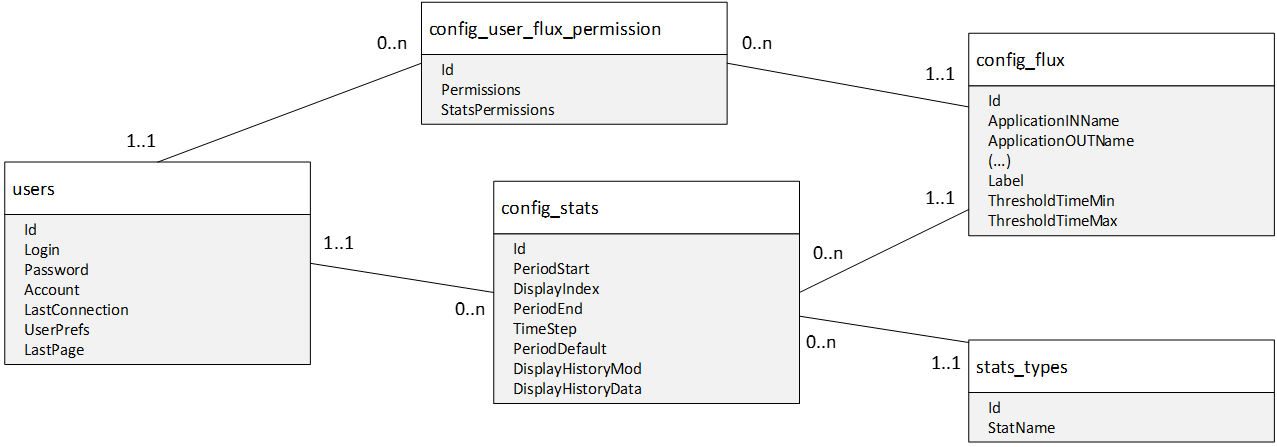
\includegraphics[width=16cm]{../img/part3/modele_donnee.png}
				\caption{\label{modele_donnee} Le nouveau modèle de donnée de TrackCIS au
				niveau du Frontal, les tables user, config\_user\_flux\_permission et
				config\_flux existent déjà dans la version actuelle de TrackCIS.}
			\end{figure}
			
			\paragraph{L'architecture du module au niveau du Frontal et de l'API :}
			Nous nous basons sur l'architecture existante et nous contentons d'ajouter
			des classes spécifiques aux statistiques dans les groupes de classes
			existant. La figure \ref{archi_stats} repend les deux schémas présentés
			précédement (les figures \ref{archi_actuelle_front} et
			\ref{archi_actuelle_api}) et montre bien que l'architecture du module
			statistique ne modifie pas les groupes de classes existantes. Le diagramme
			des classes détaillé du module statsitique est disponible en annexe 9.
			\begin{description}
				\item[Contrôleur :] Nous ajoutons une nouvelle classe de contrôleur au
				niveau du Frontal (point (a) sur la figure \ref{archi_stats}), elle sera
				spécifiquement dédiées aux statistiques. Pour l'API, nous utilisons la
				classe de contrôleur existante et nous nous contentons d'y ajouter une
				méthode dédiée au module (b)
				\item[Services :] Les classes de services sont spécifiques de chaque widget.
				Elles effectuent des traitements sur les données brutes renvoyées par
				Cloverleaf pour les rendre affichable et lisibles pour l'utilisateur. Pour
				ajouter un widget il sufit d'ajouter une classe de service au niveau de
				l'API et du Frontal ((c) et (d))
				\item[Donées :] De la même manière que les classes de services, nous créons
				une classe de donnée par widget (au niveau de
				l'API (e) et du Frontal(f)). D'autres classes de données sont communes
				a tous les widget, c'est le cas de la classe stokant les données de
				préférences d'affichage (date de début, date de fin, données à
				afficher\ldots)
				\item[Répertoires :] Nous ajoutons ici (g) deux classes : l'une permttant de
				récupérer et de mettre à jour les préférences d'affichage, l'autre
				permettant de récupérer et mettre à jour les droit de visualisation (géré
				par le champ StatPermissions de la table config\_user\_flux\_permission)
				\item[Vue :] Enfin, nous créons une page JSP dédiée à l'affichage des
				statistiques (h)
			\end{description}
			\begin{figure}[H]
				\centering
				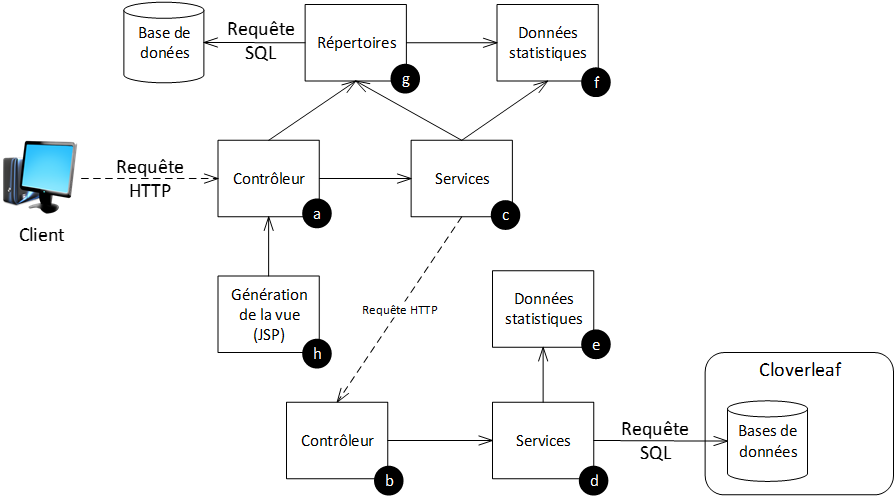
\includegraphics[width=16cm]{../img/part3/archi_stats.png}
				\caption{\label{archi_stats} La nouvelle architecture du Frontal et de
				l'API ne modifie pas l'existant.}
			\end{figure}
			
			\paragraph{La répartition des traitements :}
			Pour afficher des données lisibles et intéressantes pour les utilisateurs, il
			est nécessaire de faire des traitements sur les données brutes, comme par
			exemple :
			\begin{itemize}
			  \item Agréger les données sur un pas de temps donné (par jour, par heure\ldots)
			  \item Faire des conversions de formats de données, ce qui est notemment
			  utile pour les formats de dates
			  \item Faire des calcul de moyennes (par exmeple calculer le temps moyen de
			  transfert sur une période donnée)
			\end{itemize}
			Ces tratiements sont parfois lourd et risquent de nuire au bon fonctionnement
			de Cloverleaf. C'est pourquoi nous devons les répartir sur les différents
			niveaux de l'architecture. Les contraintes sont les suivantes :
			\begin{itemize}
			  \item L'API est déployée sur le même serveur que Cloverleaf. Pour nuire le
			  moins possible à son fonctionnement, le moins de traitements possibles
			  doivent avoir lieux à ce niveau. L'API ne doit servir qu'a extraire les
			  données brut sur la période de temps vvoulue et à les renvoyer au Frontal
			  \item Le Frontal est déployé sur un serveur dont la puissance peut être
			  très variables d'un établissement à l'autre. Tous les traitements ne
			  peuvent donc avoir lieux à ce niveaux, il devront être réparti entre le
			  Frontal et le client
			\end{itemize}
			Ce sont donc les scripts Javascript interprété au niveau du client qui vont
			être en charge d'une grande partie des traitements ainsi que de l'affichage
			des données sous forme de graphiques. Ceci est rendu possible grace à une
			bibliothèque graphique Javascript.
			
		\subsection{Réalisation des choix techniques}
			\paragraph{}% Liste des choix
			Le développement de ce projet implique l'utilisation d'un certain nombre de
			technologies. Certaines d'entre elles n'ont pas été utilisée dans la version
			actuelle de TrackCIS.
			
			\paragraph{}% Méthodo des choix
			Nous n'allons pas ici détailler tous les choix techniques qui ont été fait.
			Nous mettrons en avant dans cette partie la méthodologie avec laquelle ces
			différents choix on été effectués en l'illustrant d'un exemple, en
			l'occurence le choix de la bibliothèque graphique Javascript. Comme nous
			l'avons vu dans la partie précédente, les graphiques sont
			générés par le navigateur de l'utilisateur. Ce dernier reçois un ensemble
			de script Javascript qu'il sait interpréter. Certains de ces scripts
			permettrons d'afficher les graphiques. Pour cela nous avons besoin d'une
			bibliothèque Javascript spécifique, c'est-à-dire un ensemble de fonctions
			précrites permettant la génération de graphiques.
			Il en existe de très nombreuses et certaines sont gratuites. Pour
			faire notre choix nous partons des contraintes suivantes~:
			\begin{itemize}
			  \item La bibliothèque doit être gratuite et son utilisation pour la
			  création de produits commerciaux doit l'être également
			  \item Elle doit permettre à minima de générer les types de graphiques
			  spécifiés dans les fonctionnalités (courbe et historgamme avec plusieurs
			  séries de données, jauge et donut)
			\end{itemize}
			% Listing des librairies qui répondent à ces critères
			Nous retenons une liste de six bibliothèques qui respectent ces deux
			critères.
			Pour n'en retenir qu'une nous les comparons à l'aides d'autres critères qui
			sont~:
			\begin{itemize}
			  \item La qualité et la disponibilité de la documentation et de la
			  communauté d'utilisateur. Il est important de penser à la suite du projet
			  et aux améliorations future du module. Une bonne documentation nous
			  permettra d'aller plus vite dans le développement et également à une autre
			  équipe de s'approprier plus facilement le code pour y
			  ajouter des graphique ou corriger des bogues
			  \item L'estétisme et la possibilité de personnalier les graphiques.
			  Certaines bibliothèques proposent des graphiques prêts à l'emplois, ce qui
			  présente un gain de temps certain pour le développement. Cependant, le module
			  statistique doit respecter la charte graphique déjà en place dans l'outil,
			  les graphiques doivent donc être personnalisables au maximum
			  \item La possibilité de faire de petites animations de transition. Cela
			  peut être par exemple un petit effet à l'appartion d'une courbe, ou la
			  possibilité d'afficher une info-bulles lors du passage de la sourie sur un
			  point de donnée du graphique. Ce animations donnent vie à la visualisation
			  et améliorent l'expérience de l'utilisateur
			  \item La possibilité de pouvoir développer d'autres types de graphiques.
			  Nous ne pouvons pas prévoir comment évolura le module ni quelles nouvelles
			  données seront rendu accessibles par Cloverleaf dans l'avenir. Nous devons
			  choisir une bibliothèque nous laissant suffisament de possibilités pour
			  pouvoir créer d'autres types de visualisations
			\end{itemize}
			Tous ces critères ne sont pas égaux, certain sont plus important que
			d'autres. C'est pourquoi nous allons les pondérer à l'aide d'une note sur
			dix. Nous notons ensuite les six bibliothèques retenues sur chacun de ces
			critère, puis nous appliquons la pondération à chaque note. La note globale
			de chaque bibliothèque est le total des notes pondérées pour cahque critère.
			Le tableau \ref{choix_bib_js} présente le résultat de cette pondération.
			\begin{table}[H]
				\centering
				\caption{\label{choix_bib_js} Choix de la bibliothèque graphique
				javascript.}
				\begin{tabular}{| p{2cm} | p{2cm} | p{2cm} | p{2cm} | p{2cm} |
				p{2cm} | p{2cm} |}
					\hline
						\thead{Bibliothèque}
						&\thead{Documentation}
						&\thead{Simplicité d'utilisation}
						&\thead{Esthétisme}
						&\thead{Annimations}
						&\thead{Autres graphiques possibles}
						&\thead{Total}
						\\
					\hline
						D3&10&1&10&10&10&\thead{244}
						\\
					\hline
						Google Charts&10&9&5&5&9&\thead{230}
						\\
					\hline
						Chartist&8&6&8&10&5&\thead{202}
						\\
					\hline
						EJS Chart&7&8&7&2&8&\thead{196}
						\\
					\hline
						JQPlot&6&8&6&5&8&\thead{186}
						\\
					\hline
						RGraph&6&9&2&4&5&\thead{146}
						\\
					\hline
				\end{tabular}
			\end{table}
			La bibliothèque retenue est D3 (Data driven document), 
			open source et gratuite, elle permet de construire n'importe quel type de
			visualisation de données.
			
	\section{Une gestion de projet en mode agile}
		\paragraph{}
		La phase de conception est maintenant terminée et les choix technique
		réalisés. Nous pouvons à présent passer à l'implémentation à proprement
		parler, c'est à dire à la production du code.
		
		\subsection{Une méthode de développement ittérative}
			\paragraph{}% C'est quoi l'agilité et pourquoi ce choix
			Pour cette dernière phase nous nous inspirons des méthodes agiles, notemment
			de la méthode Scrum. La méthode Scrum est basée sur des ittérations
			successives que l'on appel les Sprints. A chaque ittération, une petite
			partie de l'application est développée et présentée au commanditaire, dans
			notre cas Xperis.
			Ceci permet d'obtenir un produit final plus proche des attentes
			du commanditaire puisque celui-ci devient un acteur à part entière du
			projet. A chaque itération il peut donner son avi sur ce qui a été
			développé et demander des améliorations ou changer ce qui avait été
			initalement prévu pour le sprint suivant.
			
			\paragraph{}% Le backlog et les US
			Le développement d'une application en sprints implique d'être en mesure de
			produire quelque chose de présentable à l'issue de chaque itération.
			Il est utile pour cela de ségmenter l'application en petites parties que
			l'on pourra développer indépendament les unes des autres : les user stories.
			Une user story correspond à un petit sénario d'utilisation de
			l'application, c'est une petite partie de l'expérience de l'utilisateur.
			Voici quelques exemples d'user stories pour notre projet :
			\begin{itemize}
			  \item En tant qu'administrateur, lors de la création d'un utilisateur, je
			  souhaite que ce dernier puisse visualiser par défaut le graphique de
			  l'historique des message pour tous les flux
			  \item En tant qu'utilisateur, je souhaite pouvoir visualiser le temps moyen
			  de transfert d'un message dans le flux de façon littérale en seconde
			  \item En tant qu'utilisateur, je souhaite pouvoir visualiser le temps
			  moyen de transfert d'un message dans le flux sur une gauge entre une
			  valeur minimum et une valeur maximum
			  \item En tant qu'utilisateur, je souhaite pouvoir consulter l'historique du
			  nombre de messages à la sortie du flux au cours du temps sous la forme
			  d'une courbe
			\end{itemize}
			
			\paragraph{}% Les sprints
			Nous choisissons des sprints d'une durée de deux semaines.Chaque sprint se
			déroule selon les étapes suivantes :
			\begin{itemize}
			  \item[1) La plannification du sprint :] Cette étape intervient au début de
			  chaque sprint. On y détermine la liste des user stories qui devront être
			  développées durant l'itération
			  \item[2) Le développement et le refactoring :] C'est la production du code
			  à proprement parler. Les user sotroies sont développées les unes après les
			  autres. Dans le temps restant à la fin du sprint il est possible de
			  retravailler le code (c'est le refactoring) pour le rendre plus lisible ou
			  pour l'optimiser
			  \item[3) La revue de code :] Cette étape se passe en fin de sprint, après
			  le développement. La revue du code s'effectue avec d'autre développeurs. Le
			  but est de discuter des améliorations qu'il est possible de faire pour
			  rendre le code plus propre et plus optimal
			  \item[4) La revue de sprint :] A la fin du sprint, on présente les users
			  stories développées au reste de l'équipe et au commanditaire. Le but est de
			  reçevoir les avis de ce dernier sur ce qui a été développé. Le
			  commanditaire peut également faire des suggestion sur ce qu'il reste à
			  développer ou demander des modifications sur ce qui a déjà été fait. Cette
			  étape permet d'adapter au mieux l'application à ce que son commanditaire en
			  attend
			  \item[5) Mise à jour de la liste des users stories :] Enfin, une fois les
			  avis du commanditaires recueillis, nous mettons a jour la liste des user
			  stories en conséquence en nous recommencons ce cycle pour le sprint suivant
			\end{itemize}
		
		\subsection{Élaboration du backlog}
			\paragraph{}% Passage des fonctionnalités aux user stories
			Le backlog est la liste des user stories. C'est à la fois un document de
			travail et de spécification.
			\begin{description}
				\item[Un document de spécification :] Le backlog est la liste exhaustive de
				tout ce que l'application est capable de faire. Une user story offre un
				niveau de détail plus fin qu'une fonctionnalité
				\item[Un document de travail :] Le backlog est l'outil central dans la
				gestion d'un projet agile. C'est lui qui est utilisé pour la plannification
				des sprints, il est mis à jour en fin d'itération après la revue de spint et
				il permet de suivre l'avancement du projet
			\end{description}
			Pour construire notre backlog, nous devont d'abord établir une liste de user
			sotries.
			De la même manière que nous avons établi le lien entre les besoins et
			les fonctionnalités, il est possible de relier ces dernières aux user
			stories.
			Une fonctionnalité peut être subdivisée en plusieurs user stories, comme le
			montre la figure \ref{mapping_fonctios_us}. Une user story n'est quant à elle
			liée qu'à une seule fonctionnalité.
			\begin{figure}[H]% Mapping fonctionnalités -> US
				\centering
				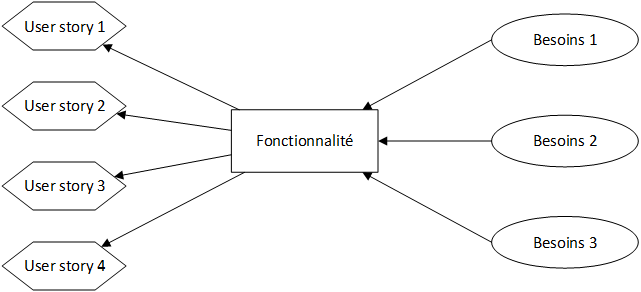
\includegraphics[width=7cm]{../img/part3/mapping_fonctios_us.png}
				\caption{\label{mapping_fonctios_us} Chaque fonctionnalité est redécoupée
				en une ou plusieurs user stories.}
			\end{figure}
			
			\paragraph{}% Priorisations des US
			L'utilisation du backlog comme outil de travail et de suivi du projet est
			rendu possible par la priorisation des éléments qui le compose. Le but de
			cette hiérarchisation est de développer en premier les user stories qui
			apportent le plus de valeur à l'utilisateur. Pour cela nous donnerons
			une note à chaque élément du backlog, note qui doit tenire compte de :
			\begin{itemize}
			  \item L'importance pour l'utilisateur de la user story, que nous
			  récupérerons en nous basant sur la note de la fonctionnalité correspondante
			  \item La difficulté de réalisation de la user story. Les users stories les
			  plus importantes sont celles qui apportent un maximum de valeur à
			  l'utilisateur tout en étant rapides à développer
			\end{itemize}
			Pour estimer la difficulté intrinsèque de chaque user story,
			nous emploirons la technique dite du planing poker. Nous utiliserons comme
			base les premiers éléments de la suite de Fibonacci (1, 2, 3, 5, 8, 13, 21,
			34,\ldots). Nous attriburons une note médianne à une user story que nous
			évaluerons de difficulté moyenne. En l'occurence nous attribuons la note de
			13 à la user story <<En tant qu'utilisateur, je souhaite voir la date et
			l'heure à laquelle le dernier message a été écrit sur ce flux>>. 
			Puis nous noterons les autres user stories relativement à la première en
			n'utilisant que des éléments de la suite de Fibonacci.\newline
			Pour obtenir la note finale de chaque user story, nous divisons simplment la
			note de la fonctionnalité correspondante par la note d'effort, comme le
			montre la formule \ref{note_us}.
			\begin{equation}
				\label{note_us}
				Note\ de\ la\ user\ story=Note\ de\ la\ fonctionnalite \times Note\ d'effort
			\end{equation}
			L'annexe 9 présente l'intégralité du backlog à la date du 4 septembre 2017.
	
	\section{Bilan de la phase de développement et suite du projet}
		\paragraph{}
		Cette dernière partie est l'occasion de faire le bilan de ce qui a été
		effectivement développé au cours de ce projet.
		
		\subsection{Les fonctionnalités implémentées}
			\paragraph{}% Bilan quantitatif de ce qui a été fait et reste à faire
			A ce stade du projet, trois sprints de deux semaines ont été complétés. Ils
			ont essentiellement portés sur le développement des deux premiers widgets :
			l'historique des messages et le temps de transfert moyen. Un total de 11 user
			stories ont été terminées, ce qui représente en tout 140 points d'effort
			(soit 16\% de la somme de tous les points d'effort du backlog). La somme des
			notes des user stories développées est de 170,55, soit 78\% de la somme de toutes
			les notes du backlog.
		
			\paragraph{Historique de nombre de messages par flux~: }
			L'utilisateur peut consulter pour chaque flux l'historique du nombre de
			message en entrée ((a) sur la figure \ref{vue_history}) et en sortie (b) du
			flux. Il peut consulter ces informations sur un graphique. Il s'agit d'une courbe avec des points de données sur
			lequel l'utilisateur peut passer le pointeur de sa sourie pour consulter des
			information détaillées (c). De plus, il peut choisir la période d'affichage
			grâce à un formulaire (d) et peut choisir de masquer l'une ou l'autre des
			séries de donnée grâce à deux boutons (e). Le pas de temps avec lequel les
			données sont agrégées et le jour.
			\begin{figure}[H]
				\centering
				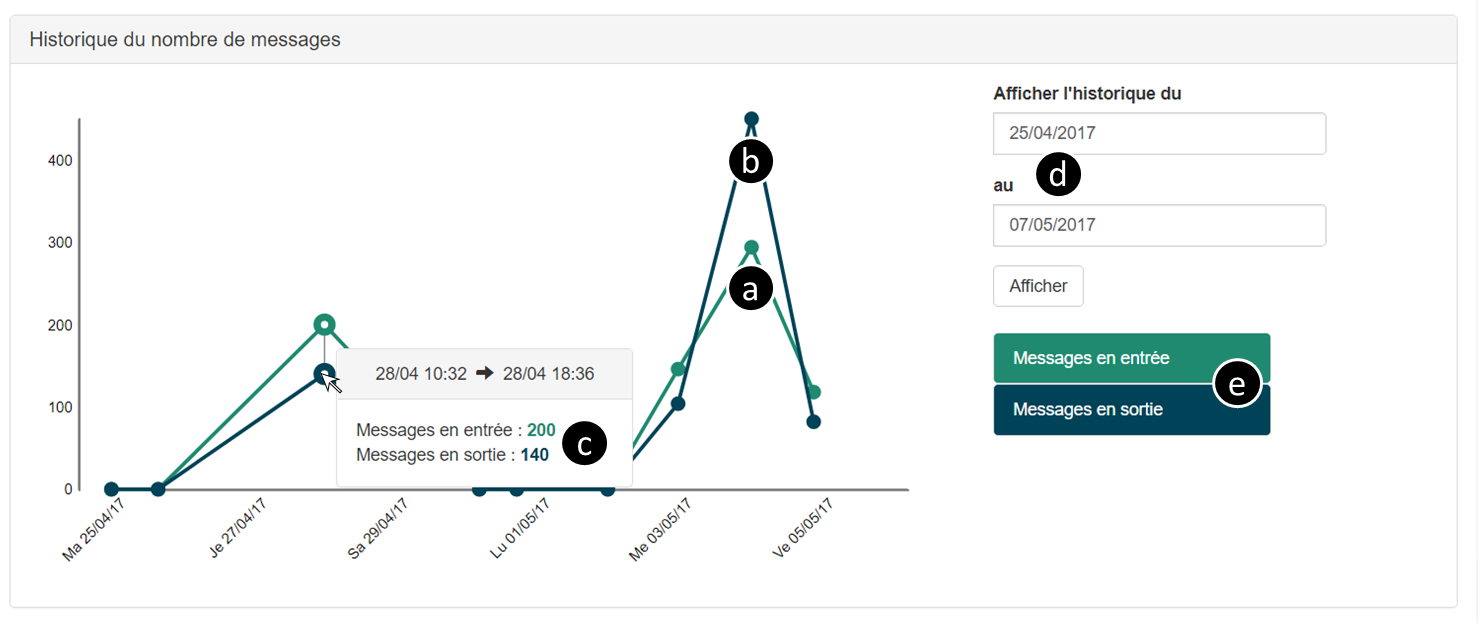
\includegraphics[width=12cm]{../img/part3/vue_history.png}
				\caption{\label{vue_history} Vue du widget historique du nombre de messages
				à ce stade du projet.}
			\end{figure}
			
			\paragraph{Valeur moyenne du temps de transfert d'un message dans le flux~: }
			L'utilisateur peut consulter le temps moyen de transfert d'un message dans
			l'EAI pour un flux donnée. Ce temps est donné en seconde ((a) sur la figure
			\ref{vue_trensfer}), il est calculé sur la base de tous les messages ayant
			transités par l'EAI sur une période donnée. L'utilisateur peut spécifier cette période graçce à un formulaire
			(b).
			\begin{figure}[H]
				\centering
				\includegraphics[width=12cm]{../img/part3/vue_trensfer.png}
				\caption{\label{vue_trensfer} Vue du widget temps de transfert à ce stade
				du projet.}
			\end{figure}
		
		\subsection{Les limites du projet}
			\paragraph{}% présentation
			Tout au long de ce prjet nous avons été amené à faire un certain nombre de
			choix, parfois de manière très arbitraire. Revenous ici sur les principales
			limites de la méthodologie globale du projet visant à améliorer TrackCIS et
			voyons comment nous pouvons en tirer les leçons pour préparer la suite du
			projet.
		
			\paragraph{}% Le choix de développer le module statistique est arbitraire
			Nous avons choisi de nous concentrer sur le développement d'un module
			d'affichage de statistiques. Rappelons que ce choix est arbitraire et est lié
			à une volonté de l'entreprise. Notre étude du besoin fait effectivement
			ressortir l'intéret des utilisateurs pour ce type de module, l'utilisation
			des statistique étant une pratique déjà existante pour tous les utilisateurs
			de Cloverleaf. Cependant cette même étude à fait ressortir d'autres besoins.
			Voici les besoins les plus importants n'ayant pas attrait aux statistiques :
			\begin{itemize}
			  \item Ouvrir l'utilisation des consoles de supervision aux personnes métier
			  \item Avoir accès à des informations sur le flux, à une documentation
			  \item Pouvoir superviser l'intégration des messages dans les applications
			  \item Pouvoir remonter directement à l'utlisateur à l'origine d'une erreur
			  de saisie
			\end{itemize}
			
			\paragraph{}% La priorisation (besoins, fonctios et US) sont aussi
			% arbitraires
			D'autre part, les méthodes que nous avons choisi pour priorier les besoins,
			les fonctionnalités et les user stories sont également arbitraires. La
			priorisation des besoin à impacté la liste des fonctionnalité de laquelle
			découle le backlog. La priorisation des user stories n'impacte que l'ordre
			dans lequel le module est développé.
			
		\subsection{Les suites possibles du projet pour Xperis}
			\paragraph{}% Les gros modules a développer à partir de l'ADB
			Les besoins que nous avons listé ci-dessus sont une bonne base pour des
			améliorationsfutures de l'outil.
			\begin{description}
				\item[Pouvoir superviser l'intégration des messages dans les applications~:]
				\item[Ouvrir l'utilisation des consoles de supervision aux personnes
				métier~:]
				\item[Avoir accès à des informations sur le flux, à une documentation~:]
				\item[Pouvoir remonter directement à l'utlisateur à l'origine d'une erreur
			  	de saisie~:]
			\end{description}
			
			\paragraph{}% Les <<petites>> amélioration à faires
			
			